% Created by tikzDevice version 0.12.3.1 on 2021-05-03 23:03:23
% !TEX encoding = UTF-8 Unicode
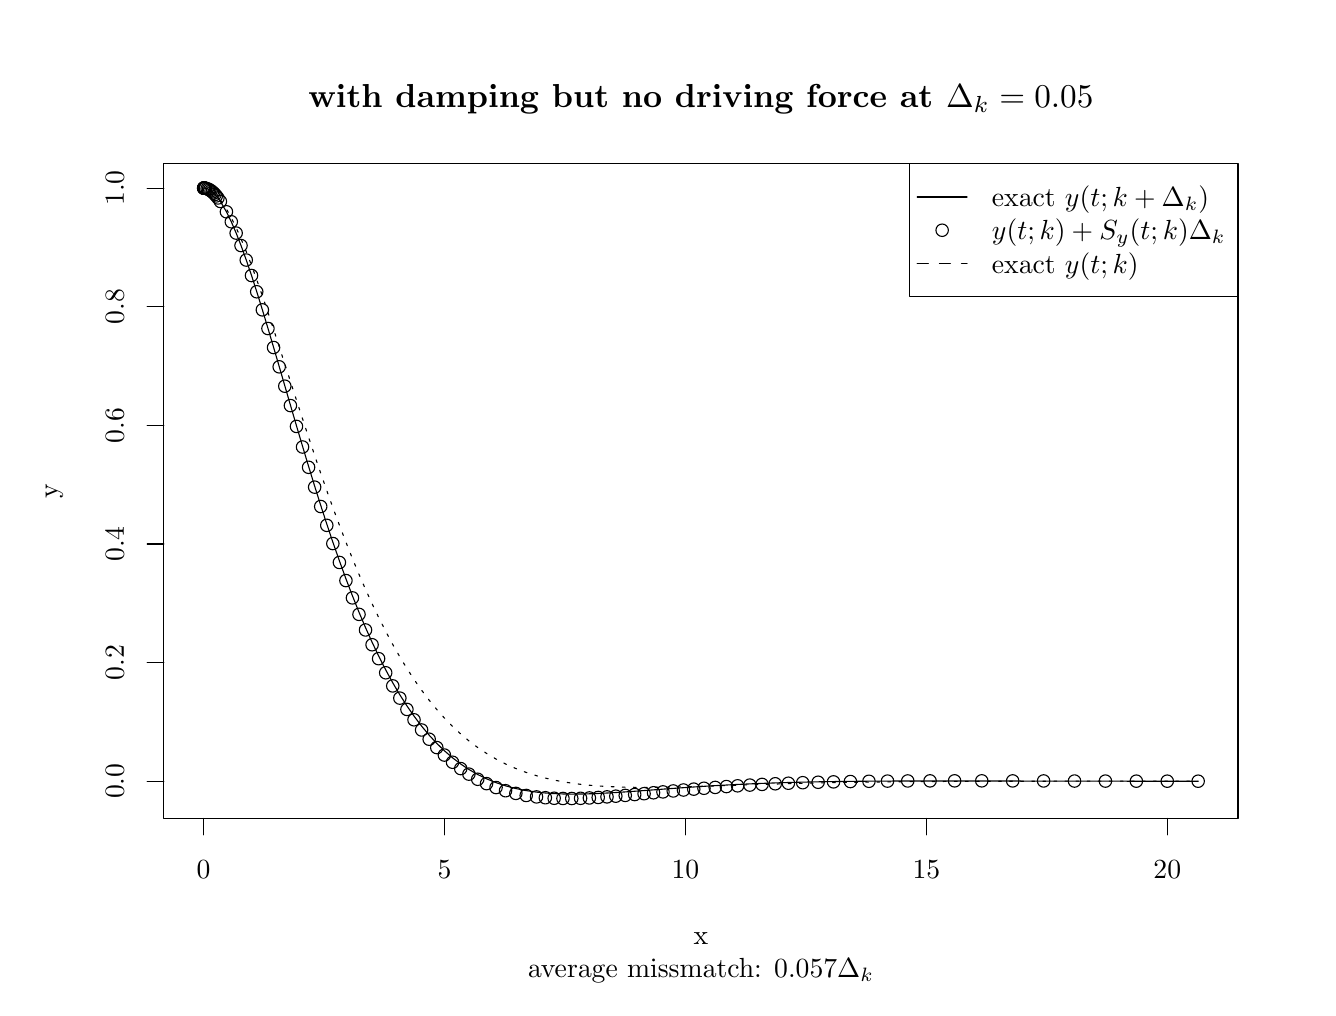
\begin{tikzpicture}[x=1pt,y=1pt]
\definecolor{fillColor}{RGB}{255,255,255}
\path[use as bounding box,fill=fillColor,fill opacity=0.00] (0,0) rectangle (462.53,346.90);
\begin{scope}
\path[clip] ( 49.20, 61.20) rectangle (437.33,297.70);
\definecolor{drawColor}{RGB}{0,0,0}

\path[draw=drawColor,line width= 0.4pt,line join=round,line cap=round] ( 63.58,288.94) --
	( 63.62,288.94) --
	( 63.66,288.94) --
	( 63.70,288.93) --
	( 63.74,288.93) --
	( 63.79,288.93) --
	( 63.88,288.92) --
	( 64.02,288.91) --
	( 64.28,288.86) --
	( 64.85,288.70) --
	( 65.32,288.50) --
	( 65.79,288.24) --
	( 66.27,287.92) --
	( 66.74,287.54) --
	( 67.21,287.11) --
	( 67.69,286.63) --
	( 68.16,286.09) --
	( 68.75,285.36) --
	( 69.64,284.10) --
	( 71.82,280.37) --
	( 73.58,276.76) --
	( 75.33,272.68) --
	( 77.09,268.19) --
	( 78.98,262.95) --
	( 80.88,257.37) --
	( 82.77,251.51) --
	( 84.80,244.99) --
	( 86.82,238.28) --
	( 88.85,231.42) --
	( 90.88,224.49) --
	( 92.91,217.51) --
	( 94.94,210.53) --
	( 97.13,203.04) --
	( 99.32,195.64) --
	(101.51,188.36) --
	(103.70,181.23) --
	(105.89,174.29) --
	(108.08,167.54) --
	(110.27,161.02) --
	(112.64,154.25) --
	(115.00,147.76) --
	(117.36,141.57) --
	(119.72,135.69) --
	(122.08,130.11) --
	(124.45,124.84) --
	(126.81,119.88) --
	(129.37,114.85) --
	(131.92,110.17) --
	(134.48,105.83) --
	(137.04,101.83) --
	(139.60, 98.14) --
	(142.34, 94.52) --
	(145.08, 91.24) --
	(147.83, 88.28) --
	(150.57, 85.62) --
	(153.52, 83.07) --
	(156.48, 80.83) --
	(159.43, 78.86) --
	(162.62, 77.03) --
	(165.81, 75.48) --
	(169.24, 74.08) --
	(172.67, 72.94) --
	(176.40, 71.96) --
	(180.14, 71.22) --
	(183.87, 70.67) --
	(187.06, 70.35) --
	(190.24, 70.13) --
	(193.42, 70.00) --
	(196.61, 69.96) --
	(199.79, 69.98) --
	(202.97, 70.06) --
	(206.16, 70.18) --
	(209.34, 70.34) --
	(212.52, 70.52) --
	(215.93, 70.74) --
	(219.34, 70.98) --
	(222.74, 71.23) --
	(226.15, 71.48) --
	(229.56, 71.74) --
	(233.27, 72.01) --
	(236.97, 72.27) --
	(240.68, 72.52) --
	(244.38, 72.76) --
	(248.43, 73.01) --
	(252.48, 73.23) --
	(256.53, 73.44) --
	(260.95, 73.64) --
	(265.36, 73.82) --
	(270.13, 73.99) --
	(274.89, 74.14) --
	(280.06, 74.27) --
	(285.63, 74.39) --
	(291.19, 74.48) --
	(297.29, 74.55) --
	(303.99, 74.62) --
	(310.70, 74.66) --
	(318.01, 74.68) --
	(326.07, 74.69) --
	(334.94, 74.69) --
	(344.76, 74.68) --
	(355.93, 74.67) --
	(367.10, 74.65) --
	(378.27, 74.63) --
	(389.44, 74.62) --
	(400.61, 74.61) --
	(411.78, 74.60) --
	(422.95, 74.60);
\end{scope}
\begin{scope}
\path[clip] (  0.00,  0.00) rectangle (462.53,346.90);
\definecolor{drawColor}{RGB}{0,0,0}

\path[draw=drawColor,line width= 0.4pt,line join=round,line cap=round] ( 63.58, 61.20) -- (411.79, 61.20);

\path[draw=drawColor,line width= 0.4pt,line join=round,line cap=round] ( 63.58, 61.20) -- ( 63.58, 55.20);

\path[draw=drawColor,line width= 0.4pt,line join=round,line cap=round] (150.63, 61.20) -- (150.63, 55.20);

\path[draw=drawColor,line width= 0.4pt,line join=round,line cap=round] (237.68, 61.20) -- (237.68, 55.20);

\path[draw=drawColor,line width= 0.4pt,line join=round,line cap=round] (324.74, 61.20) -- (324.74, 55.20);

\path[draw=drawColor,line width= 0.4pt,line join=round,line cap=round] (411.79, 61.20) -- (411.79, 55.20);

\node[text=drawColor,anchor=base,inner sep=0pt, outer sep=0pt, scale=  1.00] at ( 63.58, 39.60) {0};

\node[text=drawColor,anchor=base,inner sep=0pt, outer sep=0pt, scale=  1.00] at (150.63, 39.60) {5};

\node[text=drawColor,anchor=base,inner sep=0pt, outer sep=0pt, scale=  1.00] at (237.68, 39.60) {10};

\node[text=drawColor,anchor=base,inner sep=0pt, outer sep=0pt, scale=  1.00] at (324.74, 39.60) {15};

\node[text=drawColor,anchor=base,inner sep=0pt, outer sep=0pt, scale=  1.00] at (411.79, 39.60) {20};

\path[draw=drawColor,line width= 0.4pt,line join=round,line cap=round] ( 49.20, 74.59) -- ( 49.20,288.94);

\path[draw=drawColor,line width= 0.4pt,line join=round,line cap=round] ( 49.20, 74.59) -- ( 43.20, 74.59);

\path[draw=drawColor,line width= 0.4pt,line join=round,line cap=round] ( 49.20,117.46) -- ( 43.20,117.46);

\path[draw=drawColor,line width= 0.4pt,line join=round,line cap=round] ( 49.20,160.33) -- ( 43.20,160.33);

\path[draw=drawColor,line width= 0.4pt,line join=round,line cap=round] ( 49.20,203.20) -- ( 43.20,203.20);

\path[draw=drawColor,line width= 0.4pt,line join=round,line cap=round] ( 49.20,246.07) -- ( 43.20,246.07);

\path[draw=drawColor,line width= 0.4pt,line join=round,line cap=round] ( 49.20,288.94) -- ( 43.20,288.94);

\node[text=drawColor,rotate= 90.00,anchor=base,inner sep=0pt, outer sep=0pt, scale=  1.00] at ( 34.80, 74.59) {0.0};

\node[text=drawColor,rotate= 90.00,anchor=base,inner sep=0pt, outer sep=0pt, scale=  1.00] at ( 34.80,117.46) {0.2};

\node[text=drawColor,rotate= 90.00,anchor=base,inner sep=0pt, outer sep=0pt, scale=  1.00] at ( 34.80,160.33) {0.4};

\node[text=drawColor,rotate= 90.00,anchor=base,inner sep=0pt, outer sep=0pt, scale=  1.00] at ( 34.80,203.20) {0.6};

\node[text=drawColor,rotate= 90.00,anchor=base,inner sep=0pt, outer sep=0pt, scale=  1.00] at ( 34.80,246.07) {0.8};

\node[text=drawColor,rotate= 90.00,anchor=base,inner sep=0pt, outer sep=0pt, scale=  1.00] at ( 34.80,288.94) {1.0};

\path[draw=drawColor,line width= 0.4pt,line join=round,line cap=round] ( 49.20, 61.20) --
	(437.33, 61.20) --
	(437.33,297.70) --
	( 49.20,297.70) --
	( 49.20, 61.20);
\end{scope}
\begin{scope}
\path[clip] (  0.00,  0.00) rectangle (462.53,346.90);
\definecolor{drawColor}{RGB}{0,0,0}

\node[text=drawColor,anchor=base,inner sep=0pt, outer sep=0pt, scale=  1.20] at (243.26,318.16) {\bfseries  with damping but no driving force at $\Delta_k = 0.05$};

\node[text=drawColor,anchor=base,inner sep=0pt, outer sep=0pt, scale=  1.00] at (243.26,  3.60) {average missmatch: $0.057 \Delta_k$};

\node[text=drawColor,anchor=base,inner sep=0pt, outer sep=0pt, scale=  1.00] at (243.26, 15.60) {x};

\node[text=drawColor,rotate= 90.00,anchor=base,inner sep=0pt, outer sep=0pt, scale=  1.00] at ( 10.80,179.45) {y};
\end{scope}
\begin{scope}
\path[clip] ( 49.20, 61.20) rectangle (437.33,297.70);
\definecolor{drawColor}{RGB}{0,0,0}

\path[draw=drawColor,line width= 0.4pt,line join=round,line cap=round] ( 63.58,288.94) circle (  2.25);

\path[draw=drawColor,line width= 0.4pt,line join=round,line cap=round] ( 63.62,288.94) circle (  2.25);

\path[draw=drawColor,line width= 0.4pt,line join=round,line cap=round] ( 63.66,288.94) circle (  2.25);

\path[draw=drawColor,line width= 0.4pt,line join=round,line cap=round] ( 63.70,288.93) circle (  2.25);

\path[draw=drawColor,line width= 0.4pt,line join=round,line cap=round] ( 63.74,288.93) circle (  2.25);

\path[draw=drawColor,line width= 0.4pt,line join=round,line cap=round] ( 63.79,288.93) circle (  2.25);

\path[draw=drawColor,line width= 0.4pt,line join=round,line cap=round] ( 63.88,288.92) circle (  2.25);

\path[draw=drawColor,line width= 0.4pt,line join=round,line cap=round] ( 64.02,288.91) circle (  2.25);

\path[draw=drawColor,line width= 0.4pt,line join=round,line cap=round] ( 64.28,288.86) circle (  2.25);

\path[draw=drawColor,line width= 0.4pt,line join=round,line cap=round] ( 64.85,288.70) circle (  2.25);

\path[draw=drawColor,line width= 0.4pt,line join=round,line cap=round] ( 65.32,288.50) circle (  2.25);

\path[draw=drawColor,line width= 0.4pt,line join=round,line cap=round] ( 65.79,288.24) circle (  2.25);

\path[draw=drawColor,line width= 0.4pt,line join=round,line cap=round] ( 66.27,287.92) circle (  2.25);

\path[draw=drawColor,line width= 0.4pt,line join=round,line cap=round] ( 66.74,287.55) circle (  2.25);

\path[draw=drawColor,line width= 0.4pt,line join=round,line cap=round] ( 67.21,287.12) circle (  2.25);

\path[draw=drawColor,line width= 0.4pt,line join=round,line cap=round] ( 67.69,286.63) circle (  2.25);

\path[draw=drawColor,line width= 0.4pt,line join=round,line cap=round] ( 68.16,286.10) circle (  2.25);

\path[draw=drawColor,line width= 0.4pt,line join=round,line cap=round] ( 68.75,285.36) circle (  2.25);

\path[draw=drawColor,line width= 0.4pt,line join=round,line cap=round] ( 69.64,284.10) circle (  2.25);

\path[draw=drawColor,line width= 0.4pt,line join=round,line cap=round] ( 71.82,280.37) circle (  2.25);

\path[draw=drawColor,line width= 0.4pt,line join=round,line cap=round] ( 73.58,276.76) circle (  2.25);

\path[draw=drawColor,line width= 0.4pt,line join=round,line cap=round] ( 75.33,272.67) circle (  2.25);

\path[draw=drawColor,line width= 0.4pt,line join=round,line cap=round] ( 77.09,268.17) circle (  2.25);

\path[draw=drawColor,line width= 0.4pt,line join=round,line cap=round] ( 78.98,262.93) circle (  2.25);

\path[draw=drawColor,line width= 0.4pt,line join=round,line cap=round] ( 80.88,257.34) circle (  2.25);

\path[draw=drawColor,line width= 0.4pt,line join=round,line cap=round] ( 82.77,251.47) circle (  2.25);

\path[draw=drawColor,line width= 0.4pt,line join=round,line cap=round] ( 84.80,244.93) circle (  2.25);

\path[draw=drawColor,line width= 0.4pt,line join=round,line cap=round] ( 86.82,238.19) circle (  2.25);

\path[draw=drawColor,line width= 0.4pt,line join=round,line cap=round] ( 88.85,231.32) circle (  2.25);

\path[draw=drawColor,line width= 0.4pt,line join=round,line cap=round] ( 90.88,224.35) circle (  2.25);

\path[draw=drawColor,line width= 0.4pt,line join=round,line cap=round] ( 92.91,217.35) circle (  2.25);

\path[draw=drawColor,line width= 0.4pt,line join=round,line cap=round] ( 94.94,210.34) circle (  2.25);

\path[draw=drawColor,line width= 0.4pt,line join=round,line cap=round] ( 97.13,202.81) circle (  2.25);

\path[draw=drawColor,line width= 0.4pt,line join=round,line cap=round] ( 99.32,195.37) circle (  2.25);

\path[draw=drawColor,line width= 0.4pt,line join=round,line cap=round] (101.51,188.04) circle (  2.25);

\path[draw=drawColor,line width= 0.4pt,line join=round,line cap=round] (103.70,180.87) circle (  2.25);

\path[draw=drawColor,line width= 0.4pt,line join=round,line cap=round] (105.89,173.87) circle (  2.25);

\path[draw=drawColor,line width= 0.4pt,line join=round,line cap=round] (108.08,167.07) circle (  2.25);

\path[draw=drawColor,line width= 0.4pt,line join=round,line cap=round] (110.27,160.49) circle (  2.25);

\path[draw=drawColor,line width= 0.4pt,line join=round,line cap=round] (112.64,153.66) circle (  2.25);

\path[draw=drawColor,line width= 0.4pt,line join=round,line cap=round] (115.00,147.11) circle (  2.25);

\path[draw=drawColor,line width= 0.4pt,line join=round,line cap=round] (117.36,140.85) circle (  2.25);

\path[draw=drawColor,line width= 0.4pt,line join=round,line cap=round] (119.72,134.90) circle (  2.25);

\path[draw=drawColor,line width= 0.4pt,line join=round,line cap=round] (122.08,129.26) circle (  2.25);

\path[draw=drawColor,line width= 0.4pt,line join=round,line cap=round] (124.45,123.92) circle (  2.25);

\path[draw=drawColor,line width= 0.4pt,line join=round,line cap=round] (126.81,118.89) circle (  2.25);

\path[draw=drawColor,line width= 0.4pt,line join=round,line cap=round] (129.37,113.79) circle (  2.25);

\path[draw=drawColor,line width= 0.4pt,line join=round,line cap=round] (131.92,109.04) circle (  2.25);

\path[draw=drawColor,line width= 0.4pt,line join=round,line cap=round] (134.48,104.63) circle (  2.25);

\path[draw=drawColor,line width= 0.4pt,line join=round,line cap=round] (137.04,100.55) circle (  2.25);

\path[draw=drawColor,line width= 0.4pt,line join=round,line cap=round] (139.60, 96.80) circle (  2.25);

\path[draw=drawColor,line width= 0.4pt,line join=round,line cap=round] (142.34, 93.12) circle (  2.25);

\path[draw=drawColor,line width= 0.4pt,line join=round,line cap=round] (145.08, 89.78) circle (  2.25);

\path[draw=drawColor,line width= 0.4pt,line join=round,line cap=round] (147.83, 86.77) circle (  2.25);

\path[draw=drawColor,line width= 0.4pt,line join=round,line cap=round] (150.57, 84.06) circle (  2.25);

\path[draw=drawColor,line width= 0.4pt,line join=round,line cap=round] (153.52, 81.46) circle (  2.25);

\path[draw=drawColor,line width= 0.4pt,line join=round,line cap=round] (156.48, 79.17) circle (  2.25);

\path[draw=drawColor,line width= 0.4pt,line join=round,line cap=round] (159.43, 77.17) circle (  2.25);

\path[draw=drawColor,line width= 0.4pt,line join=round,line cap=round] (162.62, 75.31) circle (  2.25);

\path[draw=drawColor,line width= 0.4pt,line join=round,line cap=round] (165.81, 73.73) circle (  2.25);

\path[draw=drawColor,line width= 0.4pt,line join=round,line cap=round] (169.24, 72.32) circle (  2.25);

\path[draw=drawColor,line width= 0.4pt,line join=round,line cap=round] (172.67, 71.17) circle (  2.25);

\path[draw=drawColor,line width= 0.4pt,line join=round,line cap=round] (176.40, 70.20) circle (  2.25);

\path[draw=drawColor,line width= 0.4pt,line join=round,line cap=round] (180.14, 69.46) circle (  2.25);

\path[draw=drawColor,line width= 0.4pt,line join=round,line cap=round] (183.87, 68.94) circle (  2.25);

\path[draw=drawColor,line width= 0.4pt,line join=round,line cap=round] (187.06, 68.64) circle (  2.25);

\path[draw=drawColor,line width= 0.4pt,line join=round,line cap=round] (190.24, 68.45) circle (  2.25);

\path[draw=drawColor,line width= 0.4pt,line join=round,line cap=round] (193.42, 68.37) circle (  2.25);

\path[draw=drawColor,line width= 0.4pt,line join=round,line cap=round] (196.61, 68.36) circle (  2.25);

\path[draw=drawColor,line width= 0.4pt,line join=round,line cap=round] (199.79, 68.43) circle (  2.25);

\path[draw=drawColor,line width= 0.4pt,line join=round,line cap=round] (202.97, 68.56) circle (  2.25);

\path[draw=drawColor,line width= 0.4pt,line join=round,line cap=round] (206.16, 68.74) circle (  2.25);

\path[draw=drawColor,line width= 0.4pt,line join=round,line cap=round] (209.34, 68.95) circle (  2.25);

\path[draw=drawColor,line width= 0.4pt,line join=round,line cap=round] (212.52, 69.20) circle (  2.25);

\path[draw=drawColor,line width= 0.4pt,line join=round,line cap=round] (215.93, 69.48) circle (  2.25);

\path[draw=drawColor,line width= 0.4pt,line join=round,line cap=round] (219.34, 69.79) circle (  2.25);

\path[draw=drawColor,line width= 0.4pt,line join=round,line cap=round] (222.74, 70.10) circle (  2.25);

\path[draw=drawColor,line width= 0.4pt,line join=round,line cap=round] (226.15, 70.43) circle (  2.25);

\path[draw=drawColor,line width= 0.4pt,line join=round,line cap=round] (229.56, 70.75) circle (  2.25);

\path[draw=drawColor,line width= 0.4pt,line join=round,line cap=round] (233.27, 71.09) circle (  2.25);

\path[draw=drawColor,line width= 0.4pt,line join=round,line cap=round] (236.97, 71.43) circle (  2.25);

\path[draw=drawColor,line width= 0.4pt,line join=round,line cap=round] (240.68, 71.75) circle (  2.25);

\path[draw=drawColor,line width= 0.4pt,line join=round,line cap=round] (244.38, 72.06) circle (  2.25);

\path[draw=drawColor,line width= 0.4pt,line join=round,line cap=round] (248.43, 72.37) circle (  2.25);

\path[draw=drawColor,line width= 0.4pt,line join=round,line cap=round] (252.48, 72.67) circle (  2.25);

\path[draw=drawColor,line width= 0.4pt,line join=round,line cap=round] (256.53, 72.94) circle (  2.25);

\path[draw=drawColor,line width= 0.4pt,line join=round,line cap=round] (260.95, 73.21) circle (  2.25);

\path[draw=drawColor,line width= 0.4pt,line join=round,line cap=round] (265.36, 73.45) circle (  2.25);

\path[draw=drawColor,line width= 0.4pt,line join=round,line cap=round] (270.13, 73.68) circle (  2.25);

\path[draw=drawColor,line width= 0.4pt,line join=round,line cap=round] (274.89, 73.88) circle (  2.25);

\path[draw=drawColor,line width= 0.4pt,line join=round,line cap=round] (280.06, 74.07) circle (  2.25);

\path[draw=drawColor,line width= 0.4pt,line join=round,line cap=round] (285.63, 74.23) circle (  2.25);

\path[draw=drawColor,line width= 0.4pt,line join=round,line cap=round] (291.19, 74.37) circle (  2.25);

\path[draw=drawColor,line width= 0.4pt,line join=round,line cap=round] (297.29, 74.49) circle (  2.25);

\path[draw=drawColor,line width= 0.4pt,line join=round,line cap=round] (303.99, 74.58) circle (  2.25);

\path[draw=drawColor,line width= 0.4pt,line join=round,line cap=round] (310.70, 74.65) circle (  2.25);

\path[draw=drawColor,line width= 0.4pt,line join=round,line cap=round] (318.01, 74.70) circle (  2.25);

\path[draw=drawColor,line width= 0.4pt,line join=round,line cap=round] (326.07, 74.73) circle (  2.25);

\path[draw=drawColor,line width= 0.4pt,line join=round,line cap=round] (334.94, 74.74) circle (  2.25);

\path[draw=drawColor,line width= 0.4pt,line join=round,line cap=round] (344.76, 74.74) circle (  2.25);

\path[draw=drawColor,line width= 0.4pt,line join=round,line cap=round] (355.93, 74.72) circle (  2.25);

\path[draw=drawColor,line width= 0.4pt,line join=round,line cap=round] (367.10, 74.70) circle (  2.25);

\path[draw=drawColor,line width= 0.4pt,line join=round,line cap=round] (378.27, 74.67) circle (  2.25);

\path[draw=drawColor,line width= 0.4pt,line join=round,line cap=round] (389.44, 74.65) circle (  2.25);

\path[draw=drawColor,line width= 0.4pt,line join=round,line cap=round] (400.61, 74.63) circle (  2.25);

\path[draw=drawColor,line width= 0.4pt,line join=round,line cap=round] (411.78, 74.62) circle (  2.25);

\path[draw=drawColor,line width= 0.4pt,line join=round,line cap=round] (422.95, 74.61) circle (  2.25);

\path[draw=drawColor,line width= 0.4pt,dash pattern=on 1pt off 3pt ,line join=round,line cap=round] ( 63.58,288.94) --
	( 63.62,288.94) --
	( 63.66,288.94) --
	( 63.70,288.93) --
	( 63.74,288.93) --
	( 63.79,288.93) --
	( 63.88,288.93) --
	( 64.02,288.91) --
	( 64.28,288.87) --
	( 64.85,288.73) --
	( 65.32,288.55) --
	( 65.79,288.32) --
	( 66.27,288.04) --
	( 66.74,287.71) --
	( 67.21,287.33) --
	( 67.69,286.90) --
	( 68.16,286.43) --
	( 68.75,285.78) --
	( 69.64,284.67) --
	( 71.82,281.39) --
	( 73.58,278.20) --
	( 75.33,274.60) --
	( 77.09,270.63) --
	( 78.98,265.99) --
	( 80.88,261.04) --
	( 82.77,255.84) --
	( 84.80,250.03) --
	( 86.82,244.03) --
	( 88.85,237.90) --
	( 90.88,231.67) --
	( 92.91,225.39) --
	( 94.94,219.09) --
	( 97.13,212.29) --
	( 99.32,205.55) --
	(101.51,198.88) --
	(103.70,192.33) --
	(105.89,185.90) --
	(108.08,179.63) --
	(110.27,173.52) --
	(112.64,167.14) --
	(115.00,160.98) --
	(117.36,155.06) --
	(119.72,149.38) --
	(122.08,143.95) --
	(124.45,138.77) --
	(126.81,133.83) --
	(129.37,128.78) --
	(131.92,124.01) --
	(134.48,119.53) --
	(137.04,115.33) --
	(139.60,111.40) --
	(142.34,107.49) --
	(145.08,103.87) --
	(147.83,100.53) --
	(150.57, 97.45) --
	(153.52, 94.43) --
	(156.48, 91.68) --
	(159.43, 89.19) --
	(162.62, 86.79) --
	(165.81, 84.65) --
	(169.24, 82.62) --
	(172.67, 80.85) --
	(176.40, 79.19) --
	(180.14, 77.78) --
	(183.87, 76.59) --
	(187.06, 75.74) --
	(190.24, 75.01) --
	(193.42, 74.41) --
	(196.61, 73.90) --
	(199.79, 73.49) --
	(202.97, 73.16) --
	(206.16, 72.90) --
	(209.34, 72.70) --
	(212.52, 72.56) --
	(215.93, 72.46) --
	(219.34, 72.40) --
	(222.74, 72.39) --
	(226.15, 72.40) --
	(229.56, 72.44) --
	(233.27, 72.50) --
	(236.97, 72.59) --
	(240.68, 72.69) --
	(244.38, 72.79) --
	(248.43, 72.92) --
	(252.48, 73.05) --
	(256.53, 73.18) --
	(260.95, 73.32) --
	(265.36, 73.45) --
	(270.13, 73.59) --
	(274.89, 73.72) --
	(280.06, 73.85) --
	(285.63, 73.97) --
	(291.19, 74.08) --
	(297.29, 74.19) --
	(303.99, 74.29) --
	(310.70, 74.37) --
	(318.01, 74.44) --
	(326.07, 74.50) --
	(334.94, 74.54) --
	(344.76, 74.58) --
	(355.93, 74.60) --
	(367.10, 74.61) --
	(378.27, 74.62) --
	(389.44, 74.62) --
	(400.61, 74.61) --
	(411.78, 74.61) --
	(422.95, 74.61);
\definecolor{fillColor}{RGB}{255,255,255}

\path[draw=drawColor,line width= 0.4pt,line join=round,line cap=round,fill=fillColor] (318.74,297.70) rectangle (437.33,249.70);

\path[draw=drawColor,line width= 0.4pt,line join=round,line cap=round] (321.44,285.70) -- (339.44,285.70);

\path[draw=drawColor,line width= 0.4pt,dash pattern=on 4pt off 4pt ,line join=round,line cap=round] (321.44,261.70) -- (339.44,261.70);

\path[draw=drawColor,line width= 0.4pt,line join=round,line cap=round] (330.44,273.70) circle (  2.25);

\node[text=drawColor,anchor=base west,inner sep=0pt, outer sep=0pt, scale=  1.00] at (348.44,282.25) {exact $y(t;k+\Delta_k)$};

\node[text=drawColor,anchor=base west,inner sep=0pt, outer sep=0pt, scale=  1.00] at (348.44,270.25) {$y(t;k) + S_y(t;k) \Delta_k$};

\node[text=drawColor,anchor=base west,inner sep=0pt, outer sep=0pt, scale=  1.00] at (348.44,258.25) {exact $y(t;k)$};
\end{scope}
\end{tikzpicture}
